Through the earlier experimentations with the graph generations based on specific properties, improvements have been made. This includes normalisation of the values into the range of 0-10 rather than using a scale factor. Which ensures that all the graphs will be similarly shaped and have the same axis size for an easier visual comparison. Also I've included page rank as well as the other graph properties used before. Finally the datasets I will use will be generated through my program by an input of text. Afterwards will be converted into graphs where the words represent the vertices and the edges are directed to the next word in the order of the text. A factor that affected the dataset was the punctuation so to achieve congruent data, the punctuation are stripped unless they are sentence enders such as full stops, question marks, exclamation marks etc. 

Therefore, the graph we experiment on are directed graphs generated from various language families.

\section{Linguistics}
Modern languages are descendants of ancestral languages through evolution of linguistics. Through the different ages of the world, language has always been a key part in communication between societies. They are developed and taught to newer generations to reach the stages in the current world. The history of languages can be viewed as a family tree where modern languages are nearer the bottom. Along this trees, there are groups of languages that share a common ancestor. These are the \emph{language family} of those languages.
langauge
Estimations of around 500 language families exist and Campbell \cite{campbell2018many} has reported that there are exactly 406 independent language families including dead languages and \emph{language isolates} (where the language does not fit into a language family). According to Ethnologue\cite{eberhard2023a}, who are the research centre for language intelligense, there are 142 different living language families. Of the living families, six are considered to be the major families and are Indo-European, Afro-Asioatic, Niger-Congo, Austronesian, Sino-Tibetan and Trans-New Guinea.

The aim of my research is to study modern languages that fall under the Indo-European language family and the Sino-Tibetan language family. The main families are known as the \emph{proto-language} as they are the parent language where many languages are derived from\cite{rowe2022concise}. The languages being English, German and Dutch that are Germanic language under the Indo-European family. Russian and Polish which are Balto-Slavic language under Indo-European family.  French and Spanish which are Latin languages under the Indo-European language. Finally Chinese which falls under the Sino-Tibetan family. Furthermore, I will also look at Japanese which part of the Japonic language family but it would be considered a language isolate if the Ryukyuan languages were not distinct from Japanese\cite{campbell2010language}. Therefore these are all the languages in which I will translate the text extract into datasets.

\section{Text Corpus}
The best way in comparing the results to other languages is to have a dataset that is based on the same text extract. Thus, the text extract that is chosen should be simple and well know, in my case, I have chosen to use the popular story in all languages, "Sleeping Beauty". To ensure that the same version is used, the Grimm Brothers version is utilised where the original was in German and extracted from the book of children stories "Kinder- und Hausmärchen"\cite{grimm1857kinder}. So using translations of this story, graphs are generated based on each language studied.  Additionally, instead of using the entirety of the story, the first two paragraphs are used so that the graphs are not overwhelmingly dense which tells the story as follows:
\begin{quote}
In times past there lived a king and queen, who said to each other every day of their lives, "Would that we had a child!" and yet they had none. \dots There were thirteen of them in his kingdom, but as he had only provided twelve golden plates for them to eat from, one of them had to be left out.
\end{quote}
In conclusion the original nine dataset created in this way can be used for graph property calculations. Next section will study English version of the story which is part of the I

\section{Indo-European Language Family}

\subsection{English}
English words can be organised into eight different parts of speech; Nouns, Pronouns, Adjectives, Adverbs, Verbs, Prepositions, Determiners and Conjunctions. Linguistic researchers focus on the use of these categories in different situations such as through speaking or through magazines\cite{Pkhaisaeng2017study}. We will study the appearances of these categories in an extract of "Sleeping Beauty". To achieve this, the first two paragraphs of the story is received as an input in my program to achieve a usable dataset. The dataset is then converted into a directed word graph as shown by figure \ref{fig:engword}. Additionally in replacement of having each vertex labelled by the corresponding word, each vertex will be labelled with an integer and the relative integer for each word will be shown on the table of values for the graph. The table will be shown later. So we achieve the initial directed word graph both in original form and alternated form shown in figure \ref{fig:engnum}.

\begin{figure}[H]
\centering
\begin{subfigure}{.45\textwidth}
	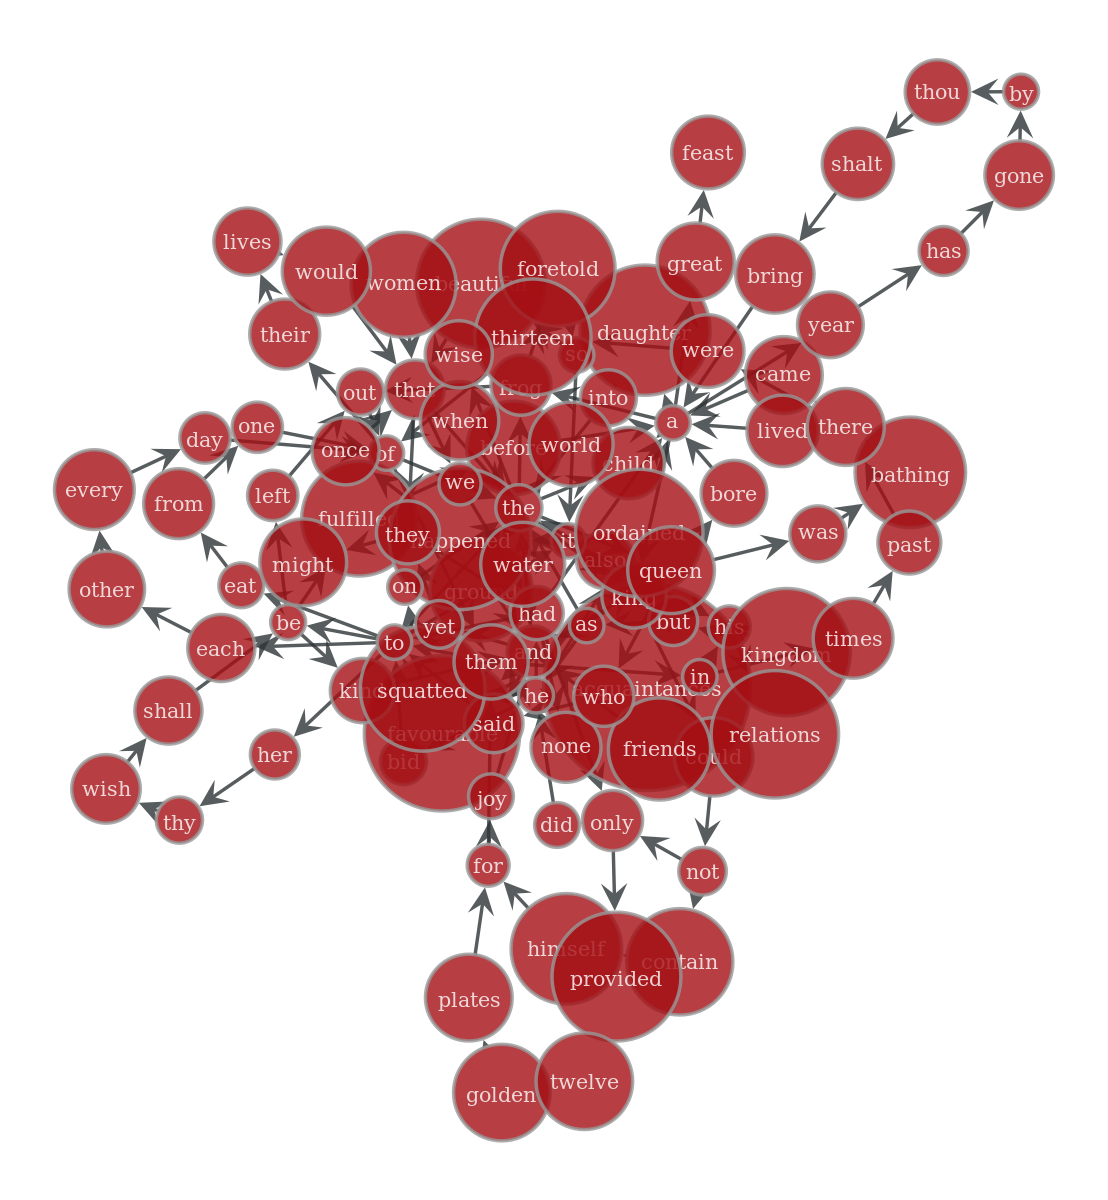
\includegraphics[scale=0.2]{englishwordgraph.png}
	\caption{Graph generated based on an extract of the story "Sleeping Beauty" with each unique word labelling each vertex.}
	\label{fig:engword}
\end{subfigure}
\hfill
\begin{subfigure}{.45\textwidth}
	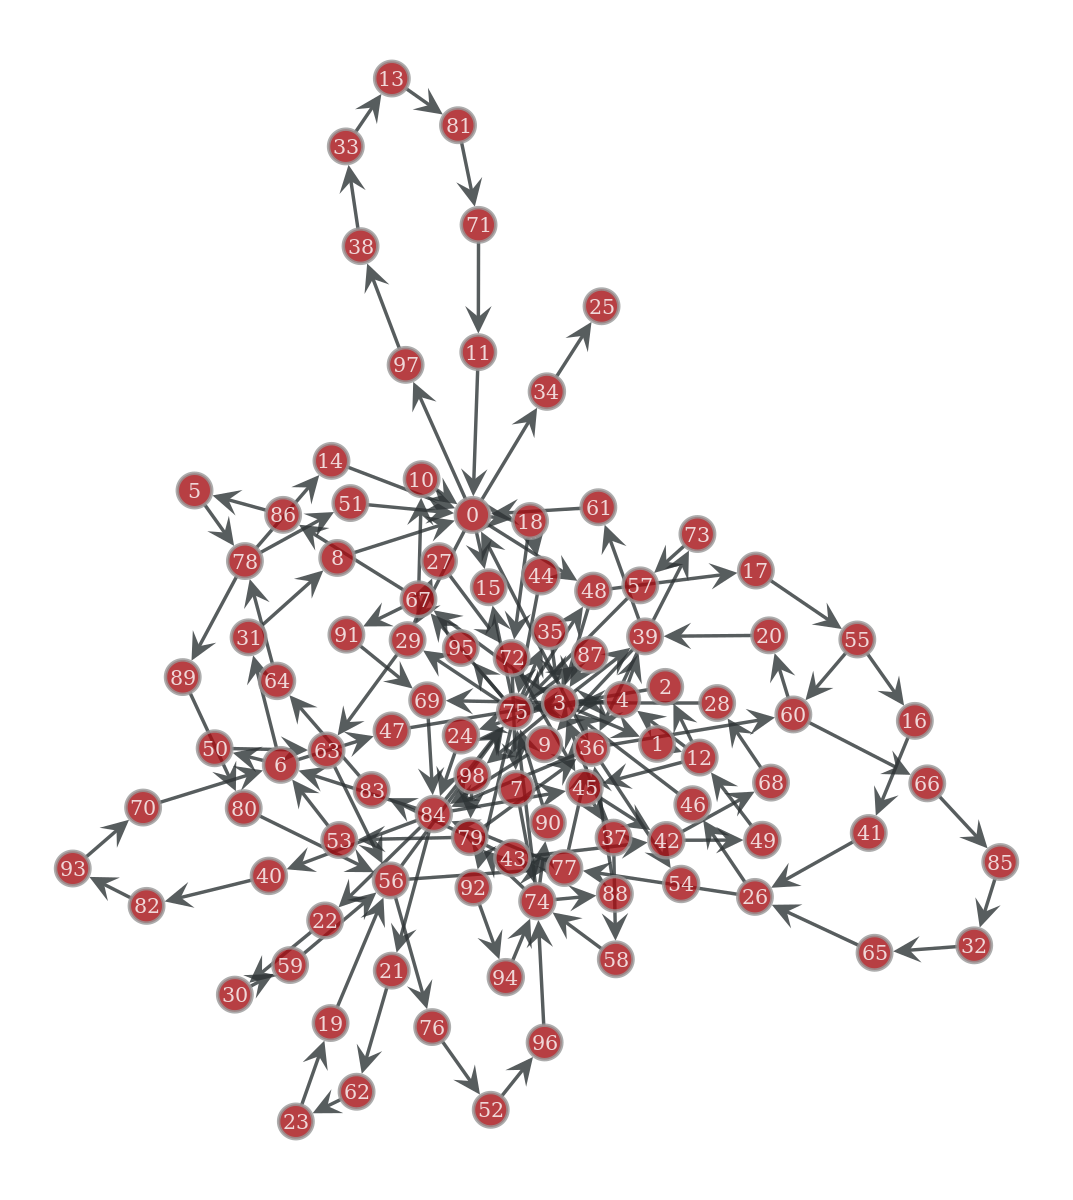
\includegraphics[scale=0.2]{englishnumbergraph.png}
	\caption{Same graph as the word graph for the English version of "Sleeping Beauty" but with numerical labelling rather than the corresponding words. The numbers are labelled in order of the unique words in alphabetical order which is also shown in the table later on.}
	\label{fig:engnum}
\end{subfigure}
\end{figure}

As done in the Early Experimentations of the karate club dataset, we calculate the values of the various graph properties explained in Chapter 2. These are graph properties such as local clustering coefficient, betweenness centrality, closeness centrality, trophic levels and page rank. Values are organised into their corresponding columns and presented as a table with the first ten entries shown in Table \ref{table:english}  below. Table also includes the number of appearances the word has denoted as count and the relative vertex number in the numbered English graph. The entire table can be seen in Appendix \ref{app:engtable}.

\begin{table}[H]
	\centering
	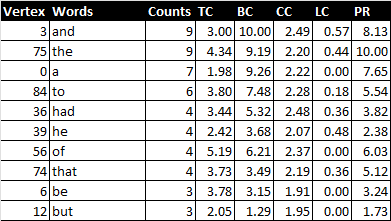
\includegraphics[scale=1]{englishtabletop10.png}
	\caption{First ten entries of the dataset generated for the english version of "Sleeping Beauty" in a table format. }
	\label{table:english}
\end{table}

We begin by analysing words with the most recurrences which are, in the order of most frequent to least, "and", "the", "a", "to", "had", "he", "of", "that", "be" and "but". Note that nouns, adverbs and adjectives do not appear in the most recurring words. These are the words that are deemed more vital in the creation of structure within a sentence. Any sentence in this story will have a high chance of containing at least one of these words. Since this is a small dataset, we can compare these words to a larger dataset for word reoccurrences as the Zipf curve for langauge are similar as discussed in a previous section. The corpus to compare to the British National Corpus (BNC)\cite{bnc2007british} which is a 100 million word collections that includes both written and spoken language. The benefits to this corpus is that it contains older English so may provide clearer correlations to the story of "Sleeping Beauty" as the Brothers Grimm version began in the late 18th century. Hence based on this corpus, the top ten frequent words\cite{leech2014word} in order of frequency are; "the", "of", "and", "a", "in", "to", "it", "is", "to" and "was". Comparing the most frequent words in both corpuses, we repetitions of words such as "the", "to" etc. Such similarities reinforce the fact that the English language has a very structured form that requires the use of these such words as the results are clear with a much smaller corpus compared to the the BNC.

Now onto the analysis of Trophic levels and coherence 

\begin{figure}[H]
\centering
\begin{subfigure}{.45\textwidth}
	\hspace{-1cm} 
	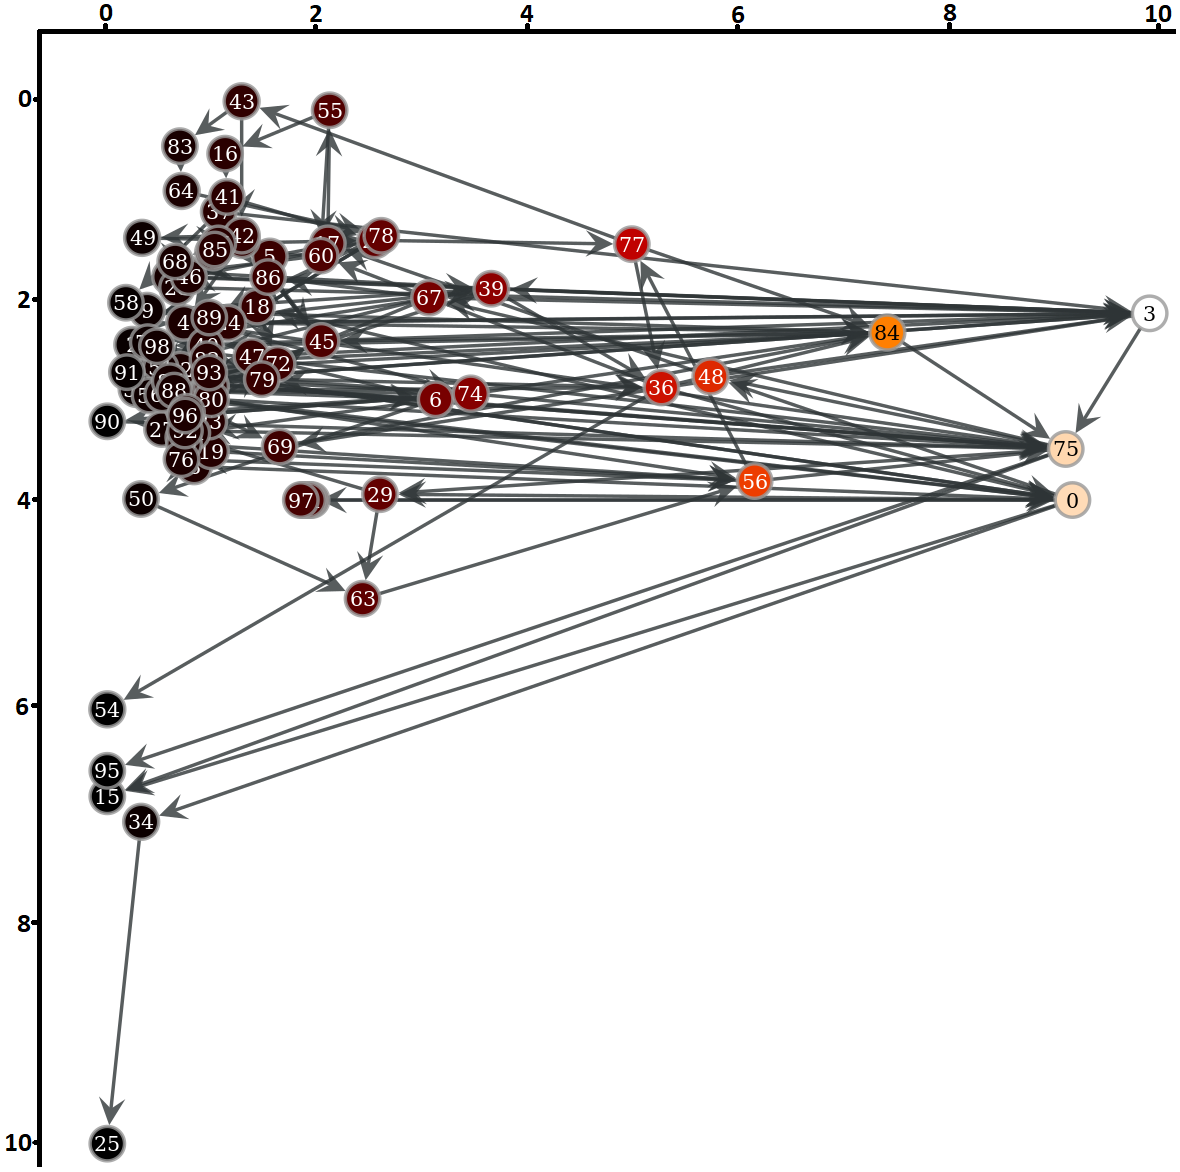
\includegraphics[scale=0.2]{englishbetweenness.png}
	\caption{}
	\label{fig:engbc}
\end{subfigure}
\hfill
\begin{subfigure}{.45\textwidth}
	\hspace{-1cm} 
	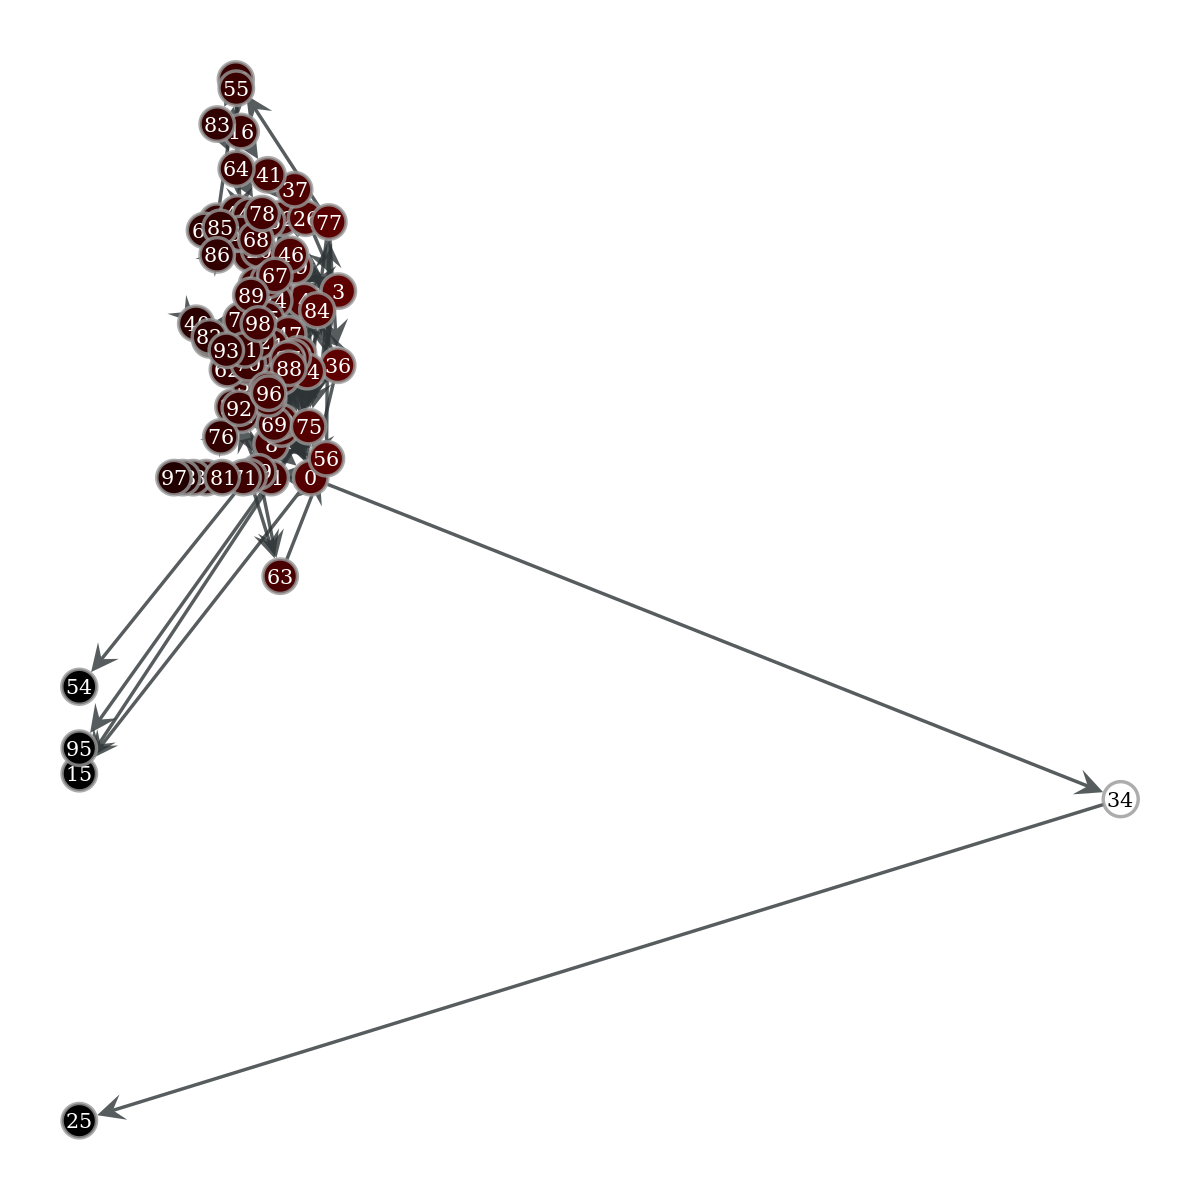
\includegraphics[scale=0.2]{englishcloseness.png}
	\caption{}
	\label{fig:engcc}
\end{subfigure}
\end{figure}

Betweenness and closeness

\begin{figure}[H]
\centering
\begin{subfigure}{.45\textwidth}
	\hspace{-1cm} 
	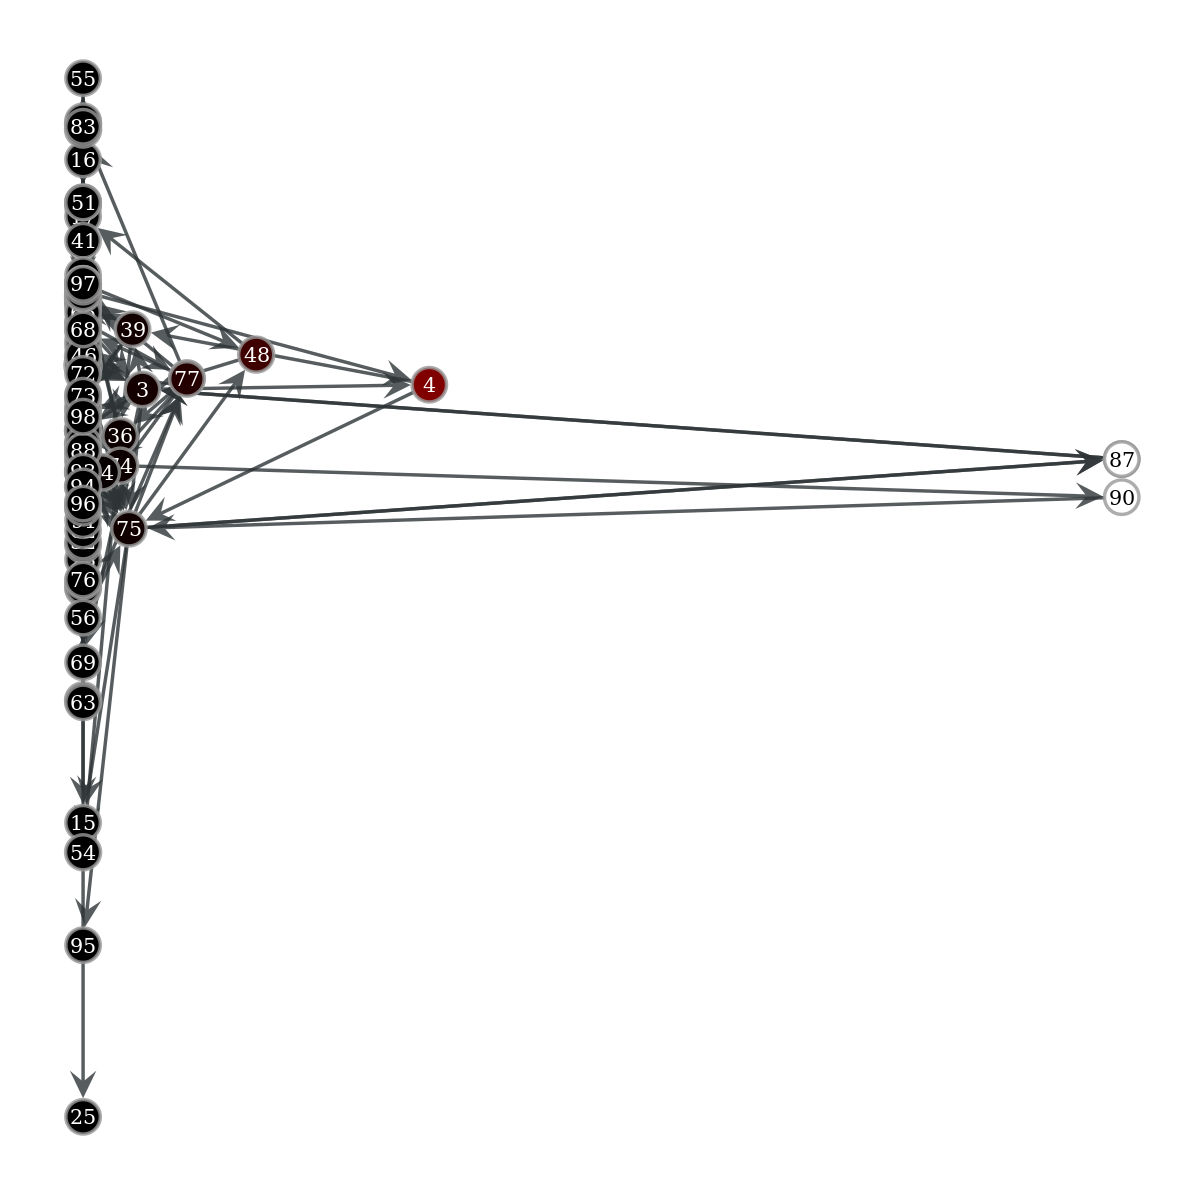
\includegraphics[scale=0.2]{englishlocalclustering.png}
	\caption{}
	\label{fig:englc}
\end{subfigure}
\hfill
\begin{subfigure}{.45\textwidth}
	\hspace{-1cm} 
	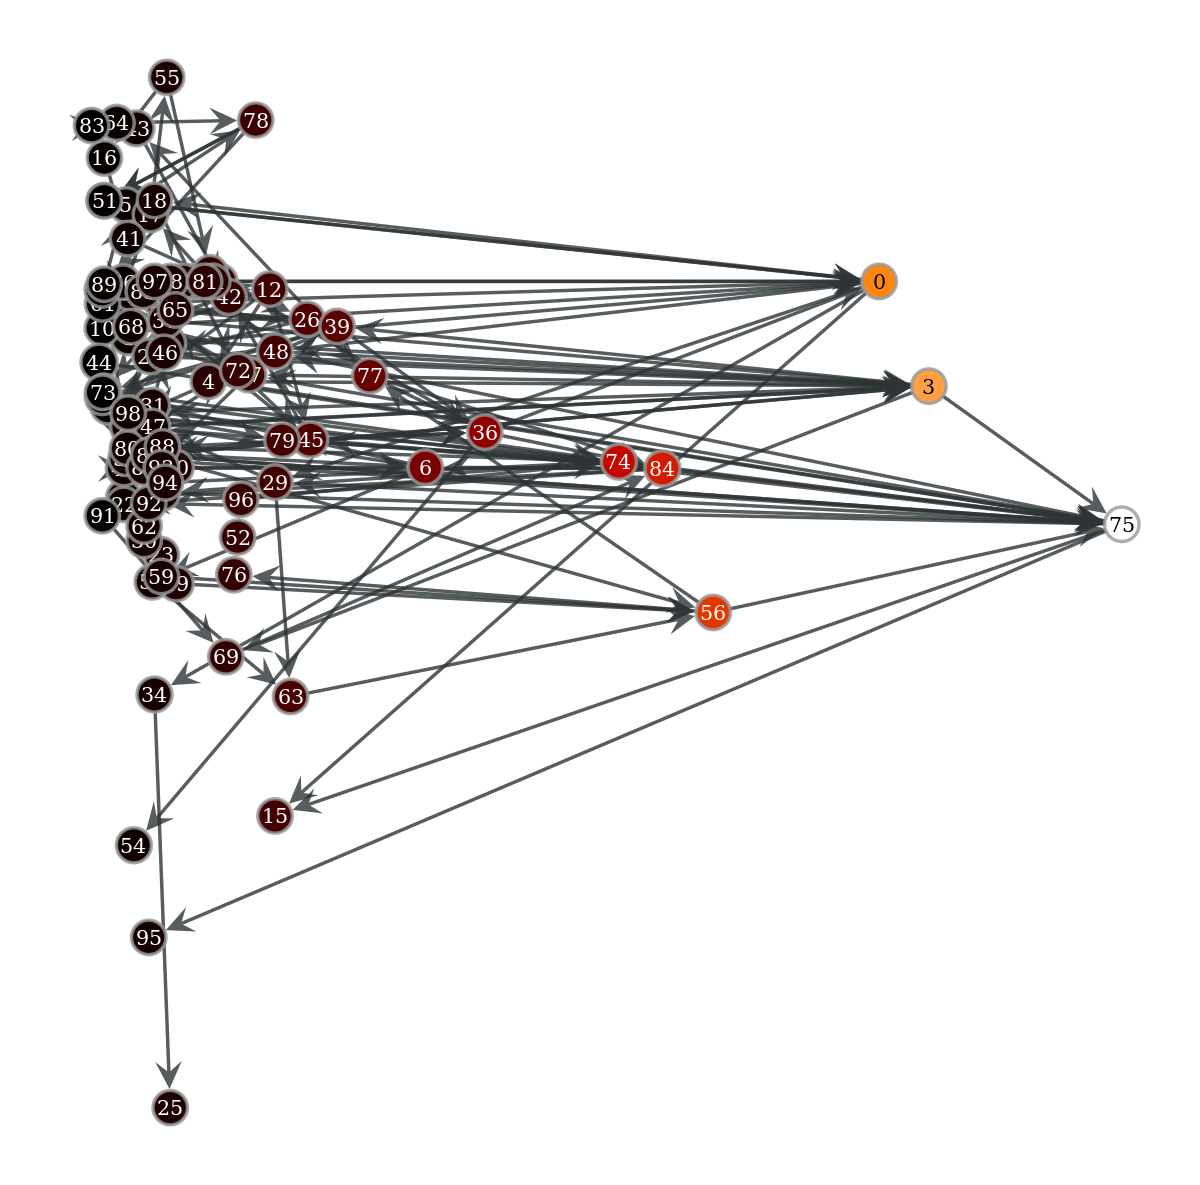
\includegraphics[scale=0.2]{englishpagerank.png}
	\caption{}
	\label{fig:engpr}
\end{subfigure}
\end{figure}

Clustering and Page rank

Conclusion
